\documentclass{article}
\usepackage{enumitem}
\usepackage{graphicx}
\usepackage{float}
\usepackage{array}


\usepackage{geometry}
 \geometry{
 a4paper,
 left=20mm,
 right=20mm
 }


\newlist{legal}{enumerate}{10}
\setlist[legal]{label*=\arabic*.}

\begin{document}
	\begin{figure}
  	
\includegraphics[width=\linewidth]{Logo-PoliMi.jpg}
	\end{figure}
\title{\textbf{RASD}}
\author{Paolo Romeo, Andrea Scotti, Francesco Staccone}
\date{AY 2018-2019}
\maketitle{}
\newpage
\textbf{Table of contents}
	\begin{legal}
 	\item Introduction
  		\begin{legal}
    		\item Purpose
		\item Scope
		\item Definitions, acronyms, abbreviations
		\item Reference documents
		\item Overview	
  		\end{legal}
	\item Overall Description
  		\begin{legal}
    		\item Product perspective
		\item Product functions
		\item User characteristics
		\item Constraints
		\item Assumptions and dependencies
  		\end{legal}
	\item Specific requirements
  		\begin{legal}
    		\item External interface requirements
		\item Functional requirements
		\item Performance requirements
		\item Design constraints
		\item Software system attributes
		\item Other requirements
  		\end{legal}
	\item Formal analysis using Alloy
  	\item Effort spent
	\item References
	\end{legal}
\newpage
	\begin{legal}\bfseries
	
 	\item {Introduction}
  		\begin{legal}\bfseries
    		\item Purpose
		\end{legal}
	{\normalfont The purpose of this document is to fully describe the TrackMe application in terms of goals, functions, requirements and constraints of the system.}
\newpage
 	\item {Overall description}
  		\begin{legal}\bfseries
    		\item Product perspective
		\end{legal}
	\begin{figure}[H]
  	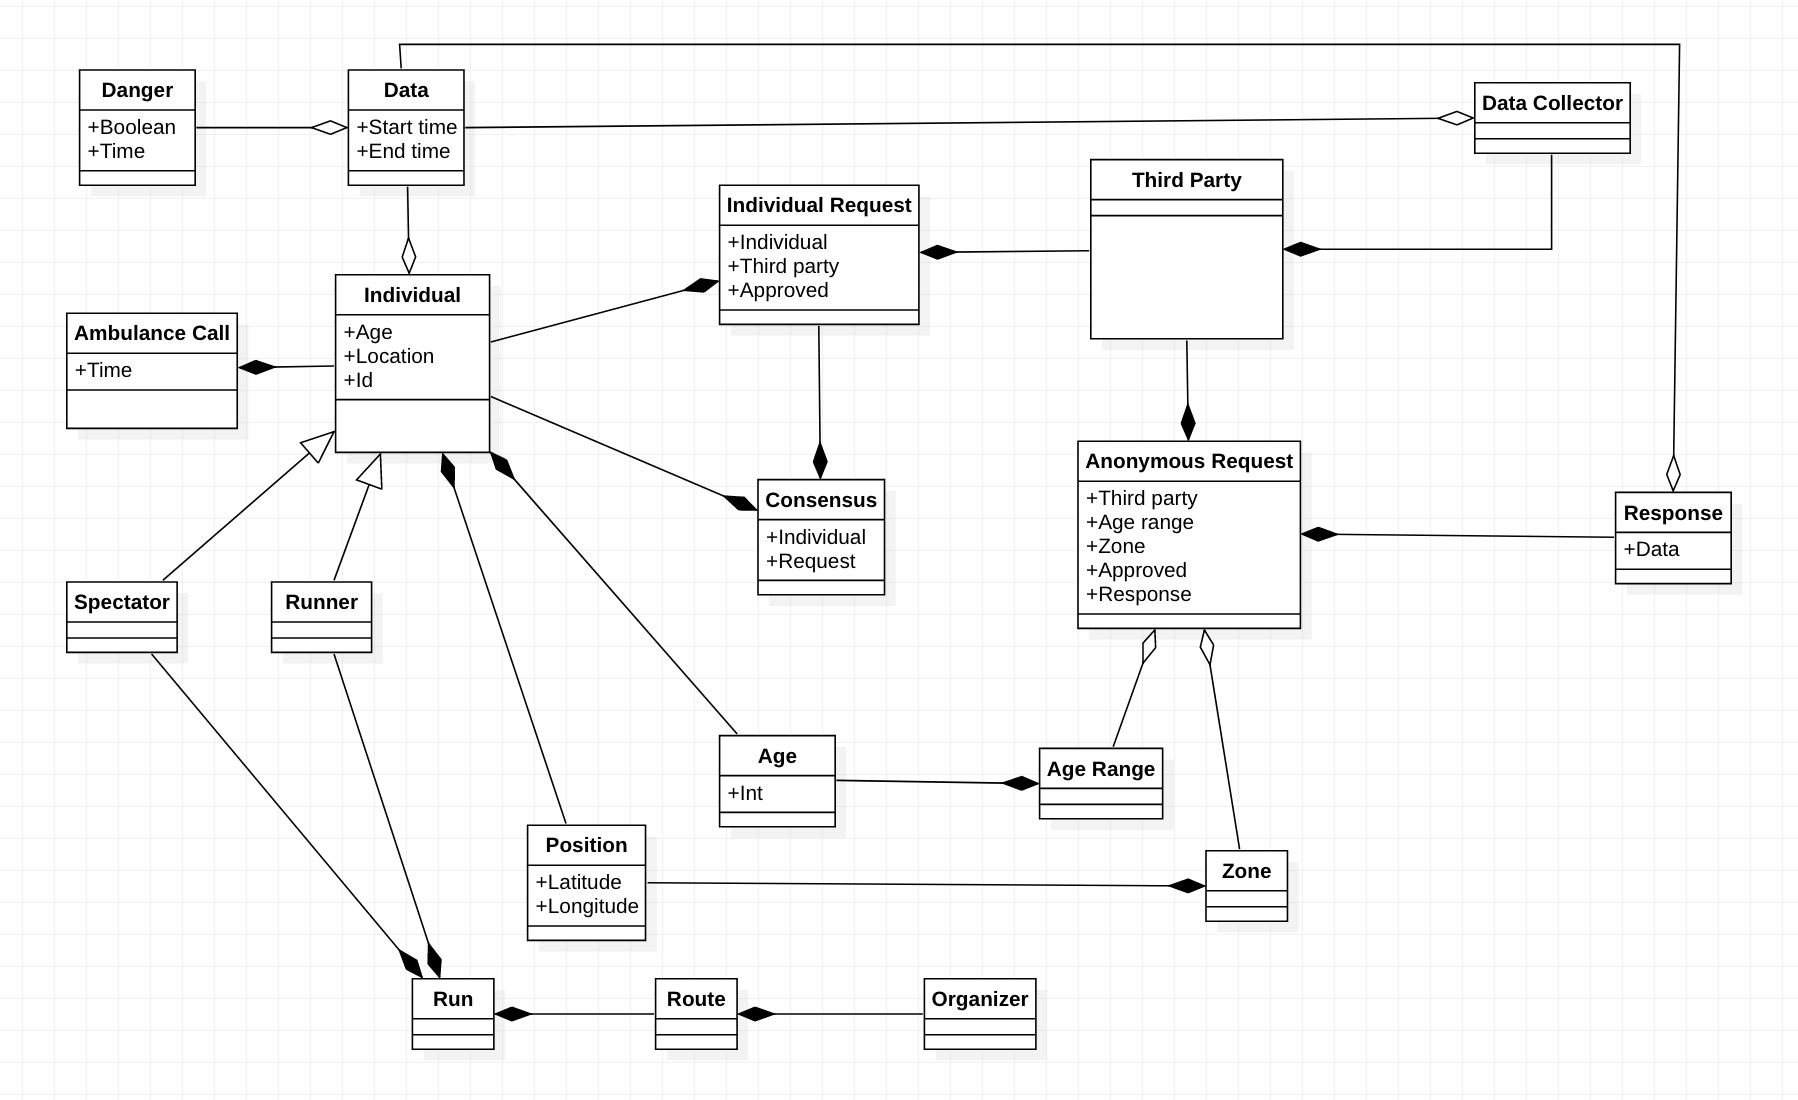
\includegraphics[width=\linewidth]{UML1-0.png}
	\end{figure}
	
	\item {Specific requirements}
  		\begin{legal}\bfseries
    		\item Functional Requirements
    		\begin{legal}\bfseries
    			\item Use Case Diagram
    			\begin{figure}[H]
			  	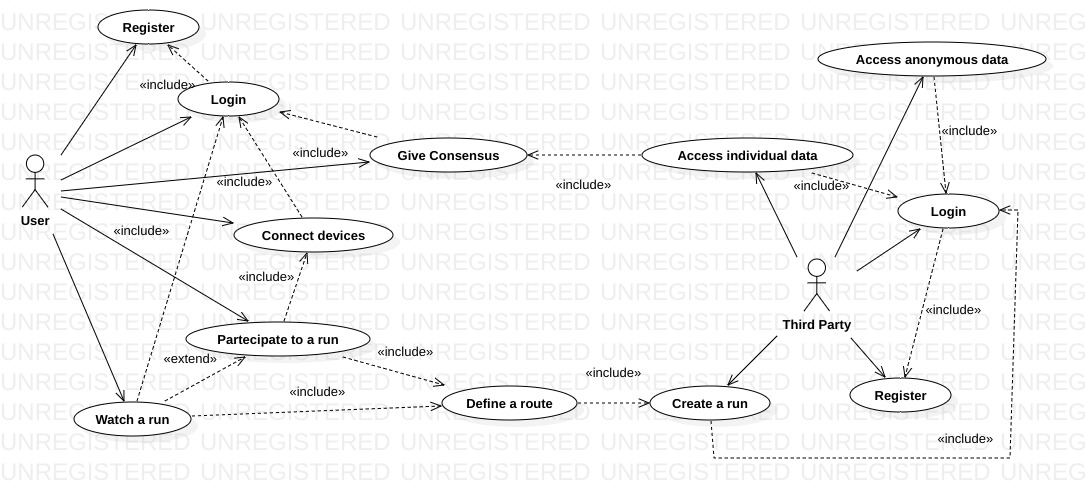
\includegraphics[width=\linewidth]{usecase.jpg}
				\end{figure}
				\item Use Case Descriptions\\\\
				\begin{tabular}{| m{3.5cm} | m{8cm}| }
				\hline
					Name & Sign up\\
				\hline
					Actor & Individual\\
				\hline
					Entry Conditions & Application installed
				on his device.\\
				\hline
					Event Flows & \begin{enumerate}
									\item The user opens the application.
									\item The user goes to the sign up session.
									
									\item The user gives all the necessary informations.
									\item The user chooses an username and a password.
									\item The user confirms his operations.
									\item The system save informations.
				\end{enumerate}\\
				\hline
					Exit Conditions & The user is successfully  registered and now he's able to log in.\\
				\hline
					Exceptions & \begin{enumerate}
									  \item The user is already registered.
									  \item The informations are incorrect or
									   missing.
				\end{enumerate}
				The user is notified and invited to try again.\\
				\hline
				\end{tabular}
				\\\\\\
				\begin{tabular}{| m{3.5cm} | m{8cm}| }
				\hline
					Name & Login\\
				\hline
					Actor & Individual\\
				\hline
					Entry Conditions & The user is previously successfully registered and has the application installed
				on his device.\\
				\hline
					Event Flows & \begin{enumerate}
									  \item The user opens the application.
									  \item The user goes to the login session.
									  \item The user inserts username and password.
									  \item The system checks if the credentials are correct.
				\end{enumerate}\\
				\hline
					Exit Conditions & The user is successfully logged in and he can access all the services. \\
				\hline
					Exceptions & The credentials are incorrect. The user is notified and invited to try again.\\
				\hline
				\end{tabular}\\\\\\
					\begin{tabular}{| m{3.5cm} | m{8cm}| }
				\hline
					Name & Connect a device\\
				\hline
					Actor & Individual\\
				\hline
					Entry Conditions & User already logged in.\\
				\hline
					Event Flows & \begin{enumerate}
									\item The user goes to the preference session.
									\item The user chooses to connect a device and then selects the right one.
				\end{enumerate}\\
				\hline
					Exit Conditions & The device is successfully connected to the application.\\
				\hline
					Exceptions & The system is not able to find or connect the device. The user is notified and invited to try again by reading carefully the connection instructions or to contact the help assistance of TrackMe.\\
				\hline
				\end{tabular}
				\\\\\\
    		\end{legal}
		\end{legal}
	
	\end{legal}
\end{document}